\chapter{Automated debugging techniques}\label{chap:automated}

\change[inline]{TODO: Link relevant literature from Slicing of~LLVM bitcode (muni.cz) and Bobox Runtime Optimization (cuni.cz)}

Debugging can be described as the~process of~analyzing erroneous code to find 
the cause of~those errors. 
Errors can also be of~different natures.
It can for example stem from poor design of~the~application.
If that is not the~case, then perhaps it comes from a~rarely
encountered input or a~corner-case. 
The flaw might also be present
in external code such as libraries or inappropriate usage of
existing technologies.

It can be said with confidence that debugging is rarely an algorithmic
app\-roach.
While the~goal is clear, the~process of~debugging depends entirely 
on the~programmer.
It is typical that developers try to look for a~root cause
of an error by feeling what might be wrong.
This works rather well in~code the~programmer is familiar with.
However, in~larger projects the~developer did not create by himself,
more sophisticated and reliable approaches are required.
For example, one might add logging to the~code being debugged,
or perhaps create more tests that can narrow down the~erroneous code.

All of~the~mentioned techniques require either the~knowledge of~the~code 
or enough time to write supporting code. Additional time might be spent
looking through the~logs and executing tests. Therefore, it is rather
hard to tell be\-fore\-hand how much time and resources debugging will take.

While most developers see debugging as a~manual chore, there were numerous 
attempts~at automating at least some parts of~it during the~last few decades. 
The rise in~popularity of~program analysis resulted in the~developement of 
automated error checkers for popular programming languages. 

SpotBugs\footnote{SpotBugs can be found at 
\url{https://spotbugs.github.io/index.html}.}, formerly known as FindBugs, 
is a~free and platform-inde\-pen\-dent application for, as the~name 
suggests, finding bugs.
It works with the~bytecode of~JDK8 and newer, which indicates that source 
code is not required.
SpotBugs uses static analysis to discover bug patterns.
These patterns are sequences of~code that might contain bugs.
They include misused language features, misused API methods, and changes to 
source code invariants created during code maintenance.
Java developers can use SpotBugs's static analysis in~its GUI form or 
as a~plugin for build tools.

Clang static analyzer\footnote{The Clang static analyzer's 
homepage is \url{https://clang-analyzer.llvm.org/}.} provides 
similar functionality to C, C++, and 
Ob\-jec\-tive-C programmers.
The code written in~these languages is parsed by the~ana\-ly\-zer.
A collection of~code analyzing techniques is then applied to it.
This process results in~an automatic bug finding, similar to compiler 
warnings.
These war\-nings, however, include runtime bugs as well.
The analyzer can uncover many bugs, from simple faulty array 
indexing to guarding the~stack address scope.
Due to its extensibility and integration in~tools and IDEs alike, 
the Clang static analyzer is popular amongst developers working 
with the~C family of~languages.

The functionality of~the~previous tool was extended 
in CodeChecker\footnote{CodeChecker's information
page is \url{https://codechecker.readthedocs.io/en/latest/}.}.
Code\-Check\-er serves as a~wrapper for the~Clang static analyzer and 
Clang-Tidy.
Wrapping these two tools into a~more sophisticated application helps 
with user-friend\-li\-ness tremendously.
Additionally, the~wrapper also deals with false positives.
Furthermore, it allows the~user to visualize the~result as HTML or 
save time by analyzing only relevant files.

Facebook's Infer\footnote{General overview of Infer can be found at 
\url{https://fbinfer.com/}.} translates both 
the C family of~languages and Java 
into a~common intermediate language.
It also utilizes compilation information for add\-itional accuracy.
The intermediate code is then analyzed one function at a~time.
During the~analysis, Infer can uncover tedious bugs such as invalid 
memory address access and thread-safety violation.

While the~tools mentioned above mainly cover only specific cases 
of potential bugs, such as out-of-range array indexing, they 
have proven themselves valuable for the~developer.
In the~context of~this work, techniques behind such checkers provide 
a~helping hand when minimizing a~program. 
Moreover, they do so with state-of-art performance.

The following sections will talk about the~techniques behind such checkers 
and how they deal with automated debugging. 
Notably, they describe the motivation and notation of~Delta debugging and 
static and dynamic slicing.

\section{Delta debugging}\label{chap:delta}

Delta debugging is an iterative approach described by Zeller\citep{Zeller99}. 
It has two primary goals for a given program and the program's 
failure-inducing input. 
The first is to simplify the input by keeping only those parts that lead to 
the failure. 
The second is to isolate a part of the input that guarantees the failure. 

The first goal is especially relevant in the context of this project and 
will be described in more detail in this section.
The simplifying algorithm, also known as the minimizing algorithm, reduces 
the size of a failure-inducing input. 
For a given program, a test case, and an input for that test case, it 
simplifies the test case's input. 
It assumes that each execution of the program has the following results: 
pass, fail, inconclusive. 

Zeller and Hildebrandt\citep*{Zeller02} have presented the following 
definitions to be more precise with the terminology.

\begin{defn}[Test case]\label{def02:1}
  Let $c_\mathcal{F}$ be a~set of~all changes $\delta_1,\dots,\delta_n$ 
  between a~passing program's input $r_\mathcal{P}$ and a~failing 
  program's input $r_\mathcal{F}$ such that 
  \begin{align}
	r_\mathcal{F} = (\delta_1(\delta_2(\dots(\delta_n(r_\mathcal{P}))))). \nonumber 
  \end{align}
  We call a~subset $c \subseteq c_\mathcal{F}$ a~\emph{test case}.
\end{defn}

To understand the definition, we must first assume two inputs for 
the debugged programs. 
Say we have an input $r_\mathcal{P}$ with which the program terminates 
successfully. 
Let us consider that the passing input is trivial, i.e., empty. 
Now consider an input $r_\mathcal{F}$ that leads to a failure when 
the program is executed. 
The difference between these two inputs is what $c_\mathcal{F}$ represents. 

The difference in the definition is decomposed into several more minor 
differences. 
In simple terms, one can think about the difference between $r_\mathcal{P}$ 
and $r_\mathcal{F}$ as the string $r_\mathcal{F}$ (since $r_\mathcal{P}$ is 
trivial). 
The decomposed differences $\delta_1, \dots, \delta_n$ represent substrings 
of the string $r_\mathcal{F}$. When composed and applied to $r_\mathcal{P}$, 
$\delta_1, \ldots, \delta_n$ transform $r_\mathcal{P}$ into $r_\mathcal{F}$. 
Subsets of ${\delta_1, \dots, \delta_n}$ are called test cases.

The goal of the minimizing algorithm is to find the minimal test case. 
The minimal test case can be interpreted as the smallest set of 
the failure-inducing input that still fails.

\begin{defn}[Global minimum]\label{def02:2}
  A~test case $c \subset c_\mathcal{F}$ is called a~\emph{global minimum}
  of~$c_\mathcal{F}$ if $\forall c_i \subseteq c_\mathcal{F}:
  (|c_i| < |c| \implies c_i$ does not cause the~program to fail.$)$
\end{defn}

The global minimum is practically impossible to compute. 
Since we are looking for a subset with specific properties, we must test 
all subsets. 
This results in exponential running time complexity. 
Instead, we can find a local minimum.

\begin{defn}[Local minimum]\label{def02:3}
  A~test case $c \subset c_\mathcal{F}$ is called a~\emph{local minimum}
  of~$c_\mathcal{F}$ if $\forall c_i \subseteq c:
  (c_i$ does not cause the~program to fail.$)$
\end{defn}

The rule for a local minimum is that no test case's subset causes failure. 
Unlike the global minimum, the local minimum is not the smallest input 
variant. 
However, it still preserves an interesting property. 
All elements of the local minimum are significant to producing the failure. 
In other words, no element can be removed.
Calculating a local minimum is also an exponentially complex operation. 
To be more efficient, we need to deploy approximations. 

\begin{defn}[$n$-minimality]\label{def02:4}
  A~test case $c \subset c_\mathcal{F}$ is \emph{$n$-minimal}
  if $\forall c_i \subseteq c:
  (|c| - |c_i| \leq n \implies c_i$ does not cause the~program to fail.$)$
\end{defn}

This approximation dictates how throughout the element removal will be. 
The larger the $n$ in $n$-minimality is, the smaller the output will be. 
Delta debugging is generally interested in $1$-minimal test cases, i.e., 
removing any element results in passing a test case. 
Though, testing for $1$-minimality might take more time than necessary.
The minimizing algorithm utilizes binary search to reduce the number of its 
iterations.

The algorithm attempts to increase its chances of finding a failing subset
by using a following modification. It tests the binary search's partitions 
as well as their complements. By testing small subsets (partitions split by
the binary search), the algorithm reduces its chances of achieving a smaller
failing test case. On the other hand, testing larger subsets (complements
of those partitions) improves the chances of finding a failing test case.
While testing larger subsets increases the chances of getting a result, it
is considerably slower.

\begin{figure}[h]
	\hrule height.8pt depth0pt \kern2pt
	\textbf{Input:} $\sigma \ldots$ the test's input string. \\
	\textbf{Output:} The reduced failure-causing substring. 
	\hrule height.8pt depth0pt \kern2pt
	\begin{algorithmic}[1]
		\State $n \leftarrow 2$
		\State Split the~string $\sigma$ into $\alpha_1,\dots,\alpha_n$ of~equal size.
		\State For each $\alpha_i$, calculate its complement $\beta_i$.
		\State Run tests on $\alpha_1,\dots,\alpha_n,\beta_1,\dots,\beta_n$.
		\If{all tests passed}
			\State $n \leftarrow 2*n$
			\If{$n > |\sigma|$}
				\Return the~most recent failure-causing substring.
			\Else
				\State goto (2).
			\EndIf
		\ElsIf{$\alpha_i failed$}
			\State $n \leftarrow 2$.
			\State $\sigma \leftarrow \alpha_i$.
			\If{$|\sigma| == 1$}
				\Return $\sigma$.
			\Else
				\State goto (2).
			\EndIf
		\Else
			\LeftComment{$\beta_i$ failed.}
			\State $\sigma \leftarrow \beta_i$.
			\State $n \leftarrow n - 1$.
			\State goto (2).
		\EndIf
	\end{algorithmic} 
	\hrule height.8pt depth0pt \kern2pt
	\caption{Minimizing Delta Debugging Algorithm.} 
	\label{alg:dd}
\end{figure}

The simplified algorithm description seen in figure~\ref{alg:dd} splits 
the~test case into $n$ even-sized partitions and their respective complements. 
These partitions are tested first, followed by all complements. 
The testing can result in~three different outcomes.
If all tests pass correctly, the~granularity, i.e., $n$, is doubled, and 
the~test case is split into more even-sized partitions. 
On the~other hand, if a~partition fails a~test, the~granularity is reset to 
its initial value.
Additionally, the~partition now becomes the~test case. 
If neither of~the~two mentioned scenarios happens, 
then a~partition's complement must have failed to pass a~test. 
This case results in~the granularity being decreased, 
and the~test case is set to the~failure causing complement.
These three steps repeat iteratively, updating the~test case and 
splitting it systematically with different granularities. 
Once the~granularity is greater than the~test cases's size, 
the most recent failure-inducing snippet is returned. 
The same case holds when the~test case is of~size $1$, i.e., it cannot be 
further divided.

For the sake of this project, we can quickly transform test case 
minimization into source code minimization:
\begin{enumerate}
  \item We consider the source code as the input of the algorithm.
  \item We compile and execute that input in an appropriate execution 
  environment.
  \item We test each iteration on whether it contains the desired runtime 
  error.
\end{enumerate}
The details on the usage of Delta debugging are described in section~
\ref{chap:deltaimplementation}.

\section{Static slicing}

Program slicing, formalized more than three decades ago,
is a~branch of~program analysis that studies program semantics.
It systematically observes and alters the~program's control-flow
and data-flow for a~given statement and variable in~the code.  
The goal of~slicing is to create a~slice of~a~program,
i.e., a~series of~parts of~the~program that could potentially
impact the~control and data flow at some given point in~that program. 
The direction from which the~target statement is approached divides 
slicing methods into two groups. 
Firstly, forward slicing uncovers parts of~the~code that 
might be affected by the~targeted statement and variable. 
Secondly, and much more common, backward slicing computes 
parts of~the~program that impacts the~targeted statement.

The first introduced slicing method was static backward slicing.
And with it came brand new formalism concerning program analysis. 
Specifically for static slicing methods, definitions for the~target 4
statement and variable needed to be written.
Weiser \citep{Weiser84}
defined a~slice with respect to criterion C 
as a~part of~a~program that potentially affects given variables in~a given point. 

\begin{defn}[Static slicing criterion]\label{def02:5}
  Let $\mathcal{P}$ be a~program consisting of~program points 
  $P = p_1,\dots,p_n$ and variables $V = v_1,\dots,v_m$.
  Any pair $C = (p_i, V')$, such that $p_i \in P$, $V' \subseteq V$, and 
  $\forall v_i \in V': v_i$ is present in~$p_i$, 
  is called a~\emph{slicing criterion}.
\end{defn}

Slicing is the~process of~finding such a~part of~a~program. 
Suggested approaches neglected any execution information and 
focused solely on observations made by analyzing the~code.

\begin{figure}[p]
\begin{minipage}{0.46\textwidth}
\begin{lstlisting}[basicstyle=\small, caption=Simple branching pro\-gram.,
  language=C++, label={lst:simpleexample}]
#include<iostream>

void write(int x)
{
	std::cout << x << "\n";
}

int read()
{
	int x;
	std::cin >> x;
	
	return x;
}

int main(void)
{
	int x = 1;
	int a = read();
	
	for (int i = 0; 
	i < 0xffff; i++)
	{
		write(i);
	}
	
	if ((a % 2) == 0)
	{
		if (a != 0)
		{
			x *= -1;
		}
		else
		{
			x = 0;
		}
	}
	else
	{
		x++;
	}

	write(x);

	return 0;
}
\end{lstlisting}
\end{minipage}
\hfill
\begin{minipage}{.45\textwidth}
\begin{lstlisting}[basicstyle=\small, caption=Static slice of~the~simple 
  branching program., language=C++, numbers=right,
  label={lst:staticslice}]
#include<iostream>

void write(int x)
{
	std::cout << x << "\n";
}

int read()
{
	int x;
	std::cin >> x;
	
	return x;
}

int main(void)
{
	int x = 1;
	int a = read();
		
	
	
	

	
	
	if ((a % 2) == 0)
	{
		if (a != 0)
		{
			x *= -1;
		}
		else
		{
			x = 0;
		}
	}
	else
	{
		x++;
	}

	write(x);

	return 0;
}
\end{lstlisting}
\end{minipage}
\caption{An illustration of the difference static slicing makes.
The source code on the left is the original program, the code on the
right is its static slice w.r.t. $C = (write(x)_{42}, \{x\})$.}
\label{lst:staticcomparison}
\end{figure}

One can imagine that the~size of~a~static slice would be much smaller
than the~original program. 
That would be the~case in~modular code that rarely interacts between
its components. 
An example of~such code would be heavy parallel applications and 
computational tasks. 
However, in~programs with aggressive use of~branching, it is not so. 
Since static slicing considers statements that \textbf{might} 
impact the~criterion, it leaves otherwise useless branches in~the slice,
thus negating the~potential decrease in~size. 

In listing~\ref{lst:simpleexample}, we can see the~code of~a~simple program.
It loads a~value $a$, which then alters the~control-flow of~the~code.
Meanwhile, it iterates through a~printing loop. 
The intriguing part, however, is the~output of~the~$write(x)$ 
command on line $42$. 
Let the~criterion be $C = (write(x)_{42}, \{x\})$. 
The value of~$x$ on that line is changed in~the branching 
part of~the~program, which entirely depends on the~value of~$a$.
Since $a$ is unknown, no significant code reduction can be made. 
The static slice with respect to $C$, seen in listing~\ref{lst:staticslice}, 
still contains all of~the~branching statements. 
Note that the~independent printing loop is gone.

Later that year, K. J. Ottenstein and L. M. Ottenstein \citep*{Ottenstein84}
restated the~problem as a~reachability
search in~the program dependence graph (PDG).
PDG represents statements in~the code as vertices and data and control
dependencies as oriented edges. 
Additionally, edges induce a~partial ordering on the~vertices. 
In order to preserve the~semantics of~the~program, statements must be executed 
according to this ordering. 

Edges are, therefore, of~two types. 
First, the~control dependency edge specifies that an incoming vertex's 
execution depends on the~outgoing one's execution. 
Second, the~data flow dependence edge suggests that a~variable appearing
in both the~outgoing and incoming edge share a~variable,
the value of~which depends on the~order of~the~vertices execution.

Once the~PDG is built, slices can be extracted in~linear time 
with respect to the~number of~vertices.

\begin{figure}[ht]\centering
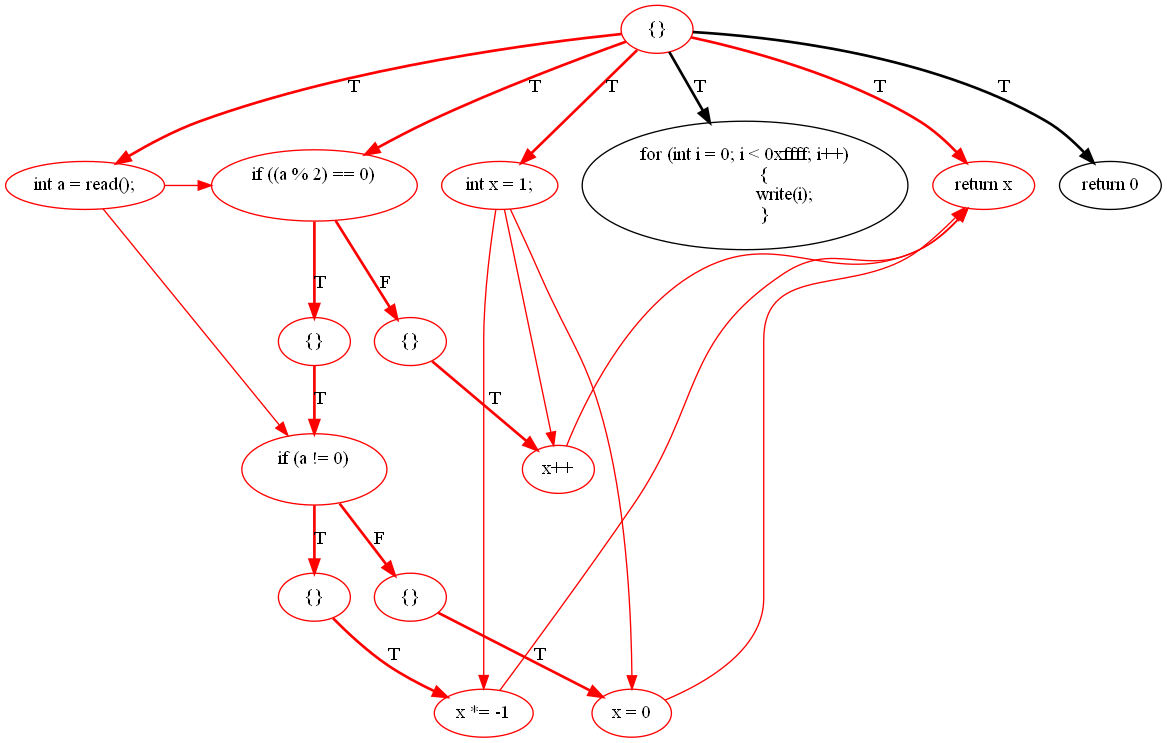
\includegraphics[scale=0.35]{pdg_sliced}
\caption{Sliced PDG. The~graph was created from the~source 
code shown in listing~\ref{lst:simpleexample}.
Red edges indicate the~sliced part of~the~program w.r.t.
$C = (write(x)_{42}, \{x\})$.}
\label{img:pdg}
\end{figure}

Figure~\ref{img:pdg} shows a~PDG that was extracted using an AST Slicer.
Nodes of~the~graph contain the~same statements as seen in~the code.
Frameworks that achieve such mapping between the~code and the~internal
control and data flows allow developers to create slicing tools much 
more easily.
One such framework is the~LLVM/Clang Tooling library, which will be
talked about later.
The tool is available at \url{https://github.com/dwat3r/slicer}.

However, one can find many potential issues and obstacles when performing 
data flow analysis. 
Omitting the~interprocedural slicing, as it is not relevant in~this projects's
context, one is left with pointers and unstructured control flow.
While the~latter is rarely used in~single-threaded modern programming, 
the same cannot be said about the~former. 

Pointers require us to extend the~syntactic data flow analysis 
into a~pointer or points-to analysis, which should be performed first. 
It is necessary to keep track of~where pointers may point to (or must point to,
in case their address is not reassigned) during the~execution. 
From this knowledge, other data flow edges must be created or
changed to accommodate the~fact when the~outgoing vertex mayhap writes
into a~memory location possibly used by the~incoming vertex. 

The analogical approach is then used for control dependency analysis since 
pointers might alter control flow as well. 
This change to control flow happens, namely when functions are called using 
function pointers.

The main advantage of~static slicing is that it does not require
any runtime information. 
As program execution can be expensive both time-wise and resource-wise, 
static slicing offers program comprehension at a~low cost. 
Because static slicing discovers program statements that can affect 
certain variables, it can remove dead code and be used for program segmentation. 

Furthermore, static slicing is used for testing software quality, maintenance, 
and test, all of~which are relevant to this project.

\section{Dynamic slicing}

While the~idea of~building a~program slice prevails, dynamic slicing 
drastically differs from static slicing in~terms of~input and the~way
it is processed. 

Korel \citep{Korel88} described a~slicing approach that took into 
consideration information regarding a~program's concrete execution. 
As opposed to static slicing, which builds a~slice for any execution, 
dynamic slicing builds a~slice for a~given execution of~a~program. 
Using information available during a~run of~the~program 
results in~a typically much smaller slice.

\begin{figure}[ht]\centering
\begin{lstlisting}[language=C++]
#include<iostream>

void write(int x)
{
	std::cout << x << "\n";
}

int read()
{
	int x;
	std::cin >> x;
	
	return x;
}

int main(void)
{
	int x = 1;
	int a = read();
		
	x = 0;

	write(x);

	return 0;
}  
\end{lstlisting}
\caption{Dynamic slice of~the~simple branching program seen
in listing~\ref{lst:simpleexample} w.r.t. 
$C = (write(x)_{42}, \{x\}, \{2\})$.}
\label{lst:dynamicslice}
\end{figure}

This decrease in~size is mainly due to removing unnecessary 
branching of~control statements and unexecuted statements in~general. 
The slicing criterion now contains a~set of~the~program's 
arguments in~addition to the~previous information. 
The location of~the~criterion's statement is also specified to avoid 
vagueness in~the execution history. 

The criterion is therefore defined as follows.

\begin{defn}[Dynamic slicing criterion]\label{def02:6}
  Let $\mathcal{H} = (s_{x1},\dots,s_{xn})$ be an execution history of~a~program 
  $\mathcal{P} = (\{s_1,\dots,s_m\}, V)$, where $s_i$ denotes a~statement
  and V is a~set of~variables $v_1,\dots,v_k$.
  Any triple $C = (h_i, V', \{a_1,\dots,a_j\})$, such that $h_i \in \mathcal{H}$,
  $V' \subseteq V$, $\forall v_i \in V': v_i$ is present in~$h_i$,
  and $\{a_1,\dots,a_j\}$ is the~input of~the~program,
  is called a~\emph{slicing criterion}.
\end{defn}

The example listing~\ref{lst:dynamicslice} was computed from the~original
listing~\ref{lst:simpleexample}. 
The criterion was set to $C = (write(x)_{42}, \{x\}, \{2\})$.
Since the~dynamic slicer witnessed the~program's execution,
it could precisely reduce the~code to only those statements
that were executed. the~result is a~significantly smaller slice
than the static slice shown in listing~\ref{lst:staticslice}.
Note that branching statements are gone.

Since dynamic slicing requires the~user to run the~program, 
it is typically used in~cases where the~execution with a~fixed 
input happens regardless. Such cases include debugging and testing. 
For debugging, dynamic slices must reflect the~subsequent restriction: 
a program and its slices must follow the~same execution paths.

\section{Summary}

While the~described program minimizing and debugging approaches have been 
formulated more than two decades ago, there have not been nearly enough 
successful attempts at implementing them. 

With each approach having its clear positives and negatives, 
it would be interesting to see how they handle program minimization. 
When cleverly used, a~combination of~these methods might 
result in~a reasonably fast and inexpensive algorithm 
for the~reduction of~program size.
